
\begin{frame}[fragile]{Polytopes}
	\pause
	A \colorit{polytope} $P$ is the convex closure of a finite number of points in $\R^n$.
	\smallskip
	\begin{center}
		\includegraphics[scale=.15]{aux/random_polytope}
	\end{center}
	
	\vskip-10pt\pause
	Its faces form a poset $\colorit{\faces(P)}$:
	\[
	F \leq G \qquad iff \qquad F \subseteq G.
	\]
	
	\pause\medskip
	
	The \colorit{linear span} of $F \in \faces(P)$ is denoted $\colorit{\Lin F}$.
\end{frame}

\begin{frame}{$f$-oriented polytopes}
	\pause
	
	Let $V$ be an $n$-dim'l vector space.
	Two ordered bases define the same \colorit{orientation} if they are related by a positive determinant $\lambda$:
	\[
	v_1 \wedge\dots\wedge v_n = \lambda \ w_1 \wedge\dots\wedge w_n.
	\]
	
	\pause\medskip
	An \colorit{$f$-orientation} on $P$ is an orientation $\beta_F$ of $\Lin F$ for each $F \in \faces(P)$.
%	 such that vertices are positively oriented.
	
	\pause\bigskip\medskip
	The \colorit{source} and \colorit{target} of a face of $P$ are defined by
	\begin{align*}
		\colorit{\so(F)} &= \set{E \mid \beta_E \wedge \normal_E^F = -\beta_F}, \\
		\colorit{\ta(F)} &= \set{E \mid \beta_E \wedge \normal_E^F = \beta_F}.
	\end{align*}
	
	%	\pause\bigskip
	%	A \colorit{thin poset orientation} on $\faces(P)$ is a label $\beta_{E \lessdot F} \in \set{+,-}$ for each cover relation in $\faces(P)$ such that
	%
	%	\[
	%	\alpha_{E \lessdot F} \cdot \alpha_{F \lessdot G} =
	%	-\alpha_{E \lessdot F'} \cdot \alpha_{F' \lessdot G}.
	%	\]
	%
	%%	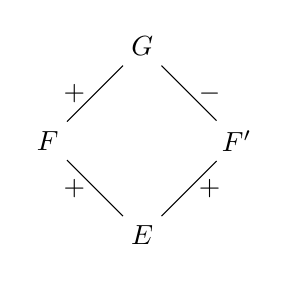
\begin{tikzpicture}[scale = .6]
	% Nodes
	\node (A) at (0,2) {$F$};
	\node (B) at (2,4) {$G$};
	\node (C) at (4,2) {$F'$};
	\node (D) at (2,0) {$E$};

	% Arrows
	\draw[-] (A) -- (B) node[midway, left] {$+$};
	\draw[-] (A) -- (D) node[midway, left] {$+$};
	\draw[-] (B) -- (C) node[midway, right] {$-$};
	\draw[-] (D) -- (C) node[midway, right] {$+$};
\end{tikzpicture}
\qquad
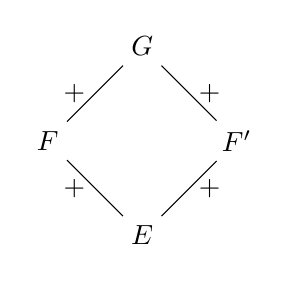
\begin{tikzpicture}[scale = .6]
	% Nodes
	\node (A) at (0,2) {$F$};
	\node (B) at (2,4) {$G$};
	\node (C) at (4,2) {$F'$};
	\node (D) at (2,0) {$E$};

	% Arrows
	\draw[-] (A) -- (B) node[midway, left] {$+$};
	\draw[-] (A) -- (D) node[midway, left] {$+$};
	\draw[-] (B) -- (C) node[midway, right] {$+$};
	\draw[-] (D) -- (C) node[midway, right] {$+$};
\end{tikzpicture}
	%	\pause\medskip
	%	\medskip\colorit{Lemma} There is a bijection between $f$-orientations on $P$ and thin poset orientations on $\faces(P)$.
\end{frame}

\begin{frame}[fragile]{Frames}
	\pause
	A \colorit{frame} is an ordered basis $\set{v_i}$ of $\R^n$:
	\begin{center}
		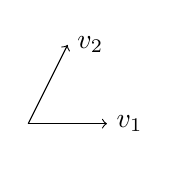
\begin{tikzpicture}
			\draw[->] (2, 0) -- (3, 0) node[anchor=west]{$v_1$};
			\draw[->] (2, 0) -- (2.5, 1) node[anchor=west]{$v_2$};
		\end{tikzpicture}
	\end{center}
	
	\pause
	It defines a filtration: \quad $0 = V_0 \leq V_1 \leq\dots\leq V_n = \R^n$
	\[
	V_k = \Span{(v_1,\ldots,v_k)}.
	\]
	
	\pause\medskip
	Its \colorit{system of projections} is the collection
	\[
	\set{\pi_k \colon \R^n \to V_k}
	\quad ; \quad
	\pi_k(v_i) =
	\begin{cases}
		v_i & i \leq k,\\
		\hfil 0 & k > i.
	\end{cases}
	\]
\end{frame}

\begin{frame}[fragile]{Framed polytopes}
	\pause
	A frame is said to be \colorit{$P$-admissible} if
	\[
	\forall F \in \faces(P),\ \pi_{\dim F}(\Lin F) = V_{\dim F}.
	\]
	We denote its inverse by $\sigma_F$.
	
	\medskip
	\colorit{Example}
	\begin{center}
		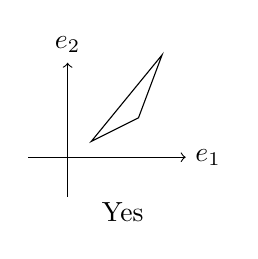
\begin{tikzpicture}
			% Draw edges
			\draw (.3,.2) -- (.9,.5) -- (1.2,1.3) -- cycle;
			
			% Draw axes
			\draw[->] (-0.5,0) -- (1.5,0) node[right] {$e_1$};
			\draw[->] (0,-0.5) -- (0,1.2) node[above] {$e_2$};
			
			\node at (.7,-.7){Yes};
		\end{tikzpicture}
		\qquad\qquad
		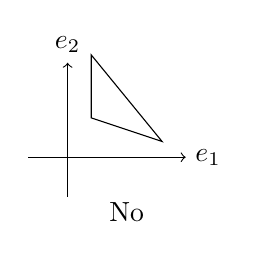
\begin{tikzpicture}
			% Draw edges
			\draw (1.2,.2) -- (.3,.5) -- (.3,1.3) -- cycle;
			
			% Draw axes
			\draw[->] (-0.5,0) -- (1.5,0) node[right] {$e_1$};
			\draw[->] (0,-0.5) -- (0,1.2) node[above] {$e_2$};
			
			\node at (.7,-.7){\;No};
		\end{tikzpicture}
	\end{center}
	
	\pause\medskip
	A polytope with a $P$-admissible is said to be \colorit{framed}.
\end{frame}

\begin{frame}{Induced $f$-orientation}
	\pause
	A $P$-admissible frame $\{v_i\}$ induces an $f$-orientation on $P$\,:
	\[
	\forall F \in \faces(P), \ \omega_F = \sigma_F v_1 \wedge\dots\wedge \sigma_F v_{\dim F}.
	\]
	
	\pause\medskip\colorit{Example}
	$(v_1, v_2)$ equivalent to $(v_1', v_2')$:
	\begin{center}
		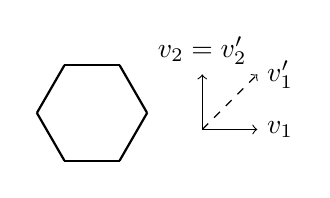
\begin{tikzpicture}[scale=.7]
			%axes
			\draw[->] (2, -.3) -- (3, -.3) node[anchor=west]{$v_1$};
			\draw[->,dashed] (2, -.3) -- (3, .7) node[anchor=west]{$v_1'$};
			\draw[->] (2, -.3) -- (2, .7) node[anchor=south]{$v_2=v_2'$};
			
			%vertices
			\node (a) at (1, 0) {};
			%\node at (1.3, 0) {$a$};
			
			\node (b) at (0.5, 0.866) {};
			%\node at (0.5, 1.2) {$b$};
			
			\node (c) at (-0.5, 0.866) {};
			%\node (c) at (-0.5, 1.2) {$c$};
			
			\node (d) at (-1, 0) {};
			%\node at (-1.3, 0) {$d$};
			
			\node (e) at (-0.5, -0.866) {};
			%\node at (-0.5, -1.2) {$e$};
			
			\node (f) at (0.5, -0.866) {};
			%\node at (0.5, -1.2) {$f$};
			
			%upper dges
			\draw[thick] (-0.5, 0.866)--(0.5, 0.866);
			\draw[thick] (1, 0)--(0.5, 0.866);
			\draw[thick] (-0.5, 0.866)--(-1, 0);
			
			%lower edges
			\draw[thick] (1,0)--(0.5, -0.866);
			\draw[thick] (-0.5, -0.866)--(0.5, -0.866);
			\draw[thick] (-0.5, -0.866)--(-1, 0) ;
		\end{tikzpicture}
	\end{center}
	
	\pause\medskip
	\colorit{Comment 1} Any $P$-admissible frame is equivalent to an orthonormal one.
	
	\pause\medskip
	\colorit{Comment 2} The \colorit{frame moduli} of an $f$-orientation $\omega$ of $P$ is satisfies Mnev's universality.
\end{frame}

%\begin{frame}{Universality}
%	\pause
%	\colorit{Question} How complicated can the moduli $\mathcal{M}(\omega)$ be?
%	
%	\pause\bigskip\medskip
%	A \colorit{semi-algebraic set} $S \subseteq \R^d$ is def'd by integral poly. eqs. and inequalities
%	\[
%	S = \set{\mathbf{x}\in\R^d \mid f_1(\mathbf{x})=0, \dots, f_k(\mathbf{x})=0, f_{k+1}(\mathbf{x})>0, \dots, f_r(\mathbf{x})>0}.
%	\]
%	
%	\pause\bigskip
%	An important relation $\sim_{\mathrm{st}}$ between them is \colorit{stable equivalence}.
%	
%	\pause\bigskip
%	\colorit{Theorem}
%	For any open semi-algebraic set $S$ there exist $n \in \N$ and an orientation $\omega$ of the $n$-simplex with $\cM(\omega) \sim_{\mathrm{st}} S$.
%\end{frame}

\begin{frame}{Extended sources and targets}
	\pause
	Let $P$ be a framed polytope.
	Its \colorit{$k$-boundary} $\bd^{(k)}(P)$ consists of its $k$-faces mapped to the boundary of $\pi_{k+1}(P)$.
	
	\pause\medskip
	It has a canonical splitting:
	\[
	\bd^{(k)}(P) = \colorit{\so_k(P)} \sqcup \colorit{\ta_k(P)}
	\]
	defined using
	\[
	\so(\pi_{k+1}(P))
	\quad\text{and}\quad
	\ta(\pi_{k+1}(P)).
	\]
	
	\pause\medskip
	Faces of a framed polytope are canonically framed, so they also have extended sources and targets.
\end{frame}

\begin{frame}{Example}
	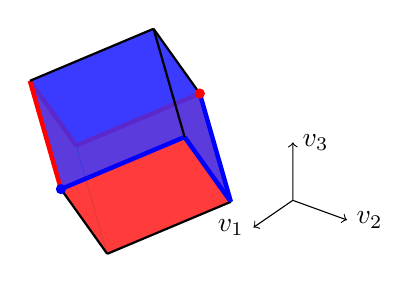
\begin{tikzpicture}%
	[x={(-0.587802cm, -0.404450cm)},
	y={(0.809005cm, -0.293947cm)},
	z={(0.000078cm, 0.866034cm)},
	scale=.850000,
	back/.style={thin, color=black!60},
	edge/.style={color=black, thick},
	sourceedge/.style={color=red, ultra thick},
	targetedge/.style={color=blue, ultra thick},
	facet/.style={fill=blue!95!black,fill opacity=0.800000},
	targetfacet/.style={fill=blue!80,fill opacity=0.800000},
	sourcefacet/.style={fill=red!80,fill opacity=0.800000},
	vertex/.style={inner sep=1pt,circle,draw=black,fill=black,thick},
	targetvertex/.style={inner sep=1pt,circle,draw=blue,fill=blue,thick},
	sourcevertex/.style={inner sep=1pt,circle,draw=red,fill=red,thick}]
	%
	%
	%% This TikZ-picture was produced with Sagemath version 10.0
	%% with the command: ._tikz_3d_in_3d and parameters:
	%% view = [-0.246900000000000, -0.484500000000000, -0.839200000000000]
	%% angle = 133.700000000000
	%% scale = 1
	%% edge_color = blue!95!black
	%% facet_color = blue!95!black
	%% opacity = 0.8
	%% vertex_color = green
	%% axis = False
	%%
	%% Coordinate of the vertices:
	%%
	\coordinate (-0.58824, 1.42857, -0.83333) at (-0.58824, 1.42857, -0.83333);
	\coordinate (0.58824, 1.42857, 0.83333) at (0.58824, 1.42857, 0.83333);
	\coordinate (1.76471, 0.00000, 0.00000) at (1.76471, 0.00000, 0.00000);
	\coordinate (0.58824, 0.00000, -1.66667) at (0.58824, 0.00000, -1.66667);
	\coordinate (-0.58824, -1.42857, -0.83333) at (-0.58824, -1.42857, -0.83333);
	\coordinate (-1.76471, 0.00000, 0.00000) at (-1.76471, 0.00000, 0.00000);
	\coordinate (-0.58824, 0.00000, 1.66667) at (-0.58824, 0.00000, 1.66667);
	\coordinate (0.58824, -1.42857, 0.83333) at (0.58824, -1.42857, 0.83333);
	%%
	%%
	%% Drawing edges in the back
	%%

	%%
	%%
	%% Drawing vertices in the back
	%%
	% \node[vertex] at (-0.58824, -1.42857, -0.83333)     {};
	%%
	%%
	\fill[targetfacet] (-0.58824, 0.00000, 1.66667) -- (0.58824, -1.42857, 0.83333) -- (-0.58824, -1.42857, -0.83333) -- (-1.76471, 0.00000, 0.00000) -- cycle {};
	\fill[sourcefacet] (-0.58824, 1.42857, -0.83333) -- (-1.76471, 0.00000, 0.00000) -- (-0.58824, -1.42857, -0.83333) -- (0.58824, 0.00000, -1.66667) -- cycle {};
	\fill[sourcefacet] (0.58824, 0.00000, -1.66667) -- (-0.58824, -1.42857, -0.83333) -- (0.58824, -1.42857, 0.83333) -- (1.76471, 0.00000, 0.00000) -- cycle {};


	\draw[edge,back] (0.58824, 0.00000, -1.66667) -- (-0.58824, -1.42857, -0.83333);
	\draw[back,sourceedge] (-0.58824, -1.42857, -0.83333) -- (-1.76471, 0.00000, 0.00000);
	\draw[back,sourceedge] (-0.58824, -1.42857, -0.83333) -- (0.58824, -1.42857, 0.83333);

	% %% Drawing the facets
	% %%
	\fill[sourcefacet] (0.58824, 0.00000, -1.66667) -- (-0.58824, 1.42857, -0.83333) -- (0.58824, 1.42857, 0.83333) -- (1.76471, 0.00000, 0.00000) -- cycle {};
	\fill[targetfacet] (0.58824, -1.42857, 0.83333) -- (1.76471, 0.00000, 0.00000) -- (0.58824, 1.42857, 0.83333) -- (-0.58824, 0.00000, 1.66667) -- cycle {};
	\fill[targetfacet] (-0.58824, 0.00000, 1.66667) -- (0.58824, 1.42857, 0.83333) -- (-0.58824, 1.42857, -0.83333) -- (-1.76471, 0.00000, 0.00000) -- cycle {};
	%%
	%%
	%% Drawing edges in the front
	%%
	\draw[targetedge] (-0.58824, 1.42857, -0.83333) -- (0.58824, 1.42857, 0.83333);
	\draw[edge] (-0.58824, 1.42857, -0.83333) -- (0.58824, 0.00000, -1.66667);
	\draw[targetedge] (-0.58824, 1.42857, -0.83333) -- (-1.76471, 0.00000, 0.00000);
	\draw[targetedge] (0.58824, 1.42857, 0.83333) -- (1.76471, 0.00000, 0.00000);
	\draw[edge] (0.58824, 1.42857, 0.83333) -- (-0.58824, 0.00000, 1.66667);
	\draw[edge] (1.76471, 0.00000, 0.00000) -- (0.58824, 0.00000, -1.66667);
	\draw[sourceedge] (1.76471, 0.00000, 0.00000) -- (0.58824, -1.42857, 0.83333);
	\draw[edge] (-1.76471, 0.00000, 0.00000) -- (-0.58824, 0.00000, 1.66667);
	\draw[edge] (-0.58824, 0.00000, 1.66667) -- (0.58824, -1.42857, 0.83333);
	%%
	%%
	% %% Drawing the vertices in the front
	% %%
	% \node[vertex] at (-0.58824, 1.42857, -0.83333)     {};
	% \node[vertex] at (0.58824, 1.42857, 0.83333)     {};
	\node[targetvertex] at (1.76471, 0.00000, 0.00000)     {};
	% \node[vertex] at (0.58824, 0.00000, -1.66667)     {};
	\node[sourcevertex] at (-1.76471, 0.00000, 0.00000)     {};
	% \node[vertex] at (-0.58824, 0.00000, 1.66667)     {};
	% \node[vertex] at (0.58824, -1.42857, 0.83333)     {};
	% %%
	% %%
	% %
	\begin{scope}[shift={(0,3,0)}]

		%axes
		\draw[->] (0, 0,0) -- (1, 0,0) node[anchor=east]{$v_1$};
		\draw[->] (0, 0,0) -- (0, 1,0) node[anchor=west]{$v_2$};
		\draw[->] (0, 0,0) -- (0, 0, 1) node[anchor=west]{$v_3$};
	\end{scope}

\end{tikzpicture}
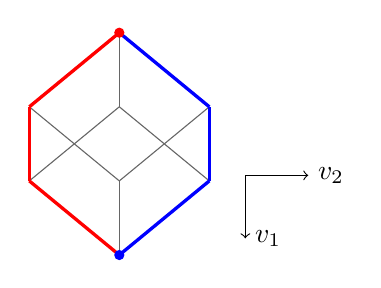
\begin{tikzpicture}%
	[
	x={(0.000000cm, -1.000000cm)},
	y={(1.000000cm, 0.000000cm)},
	z={(0.000000cm, 0.000000cm)},
	scale=.8,
	back/.style={thin, color=black!60},
	edge/.style={color=black, thick},
	sourceedge/.style={color=red, very thick},
	targetedge/.style={color=blue, very thick},
	facet/.style={fill=blue!95!black,fill opacity=0.800000},
	targetfacet/.style={fill=blue,fill opacity=0.600000},
	sourcefacet/.style={fill=red,fill opacity=0.600000},
	vertex/.style={inner sep=1pt,circle,draw=black,fill=black,thick},
	targetvertex/.style={inner sep=1pt,circle,draw=blue,fill=blue,thick},
	sourcevertex/.style={inner sep=1pt,circle,draw=red,fill=red,thick}]

\coordinate (-0.58824, 1.42857, -0.83333) at (-0.58824, 1.42857, -0.83333);
\coordinate (0.58824, 1.42857, 0.83333) at (0.58824, 1.42857, 0.83333);
\coordinate (1.76471, 0.00000, 0.00000) at (1.76471, 0.00000, 0.00000);
\coordinate (0.58824, 0.00000, -1.66667) at (0.58824, 0.00000, -1.66667);
\coordinate (-0.58824, -1.42857, -0.83333) at (-0.58824, -1.42857, -0.83333);
\coordinate (-1.76471, 0.00000, 0.00000) at (-1.76471, 0.00000, 0.00000);
\coordinate (-0.58824, 0.00000, 1.66667) at (-0.58824, 0.00000, 1.66667);
\coordinate (0.58824, -1.42857, 0.83333) at (0.58824, -1.42857, 0.83333);

\draw[edge,back] (-0.58824, 1.42857, -0.83333) -- (0.58824, 0.00000, -1.66667);
\draw[edge,back] (1.76471, 0.00000, 0.00000) -- (0.58824, 0.00000, -1.66667);
\draw[edge,back] (0.58824, 0.00000, -1.66667) -- (-0.58824, -1.42857, -0.83333);

\draw[edge,back] (0.58824, 1.42857, 0.83333) -- (-0.58824, 0.00000, 1.66667);
\draw[edge,back] (-1.76471, 0.00000, 0.00000) -- (-0.58824, 0.00000, 1.66667);
\draw[edge,back] (-0.58824, 0.00000, 1.66667) -- (0.58824, -1.42857, 0.83333);

\draw[back,sourceedge] (-0.58824, -1.42857, -0.83333) -- (-1.76471, 0.00000, 0.00000);
\draw[back,sourceedge] (-0.58824, -1.42857, -0.83333) -- (0.58824, -1.42857, 0.83333);
\draw[targetedge] (-0.58824, 1.42857, -0.83333) -- (0.58824, 1.42857, 0.83333);
\draw[targetedge] (-0.58824, 1.42857, -0.83333) -- (-1.76471, 0.00000, 0.00000);
\draw[targetedge] (0.58824, 1.42857, 0.83333) -- (1.76471, 0.00000, 0.00000);
\draw[sourceedge] (1.76471, 0.00000, 0.00000) -- (0.58824, -1.42857, 0.83333);
\node[targetvertex] at (1.76471, 0.00000, 0.00000)     {};
\node[sourcevertex] at (-1.76471, 0.00000, 0.00000)     {};
\begin{scope}[shift={(.5,2,0)}]
	\draw[->] (0, 0,0) -- (1, 0,0) node[anchor=west]{$v_1$};
	\draw[->] (0, 0,0) -- (0, 1,0) node[anchor=west]{$v_2$};
\end{scope}
\end{tikzpicture}
\begin{tikzpicture}%
	[scale=.8,
	back/.style={thin, color=black!60},
	edge/.style={color=black, thick},
	sourceedge/.style={color=red, very thick},
	targetedge/.style={color=blue, very thick},
	facet/.style={fill=blue!95!black,fill opacity=0.800000},
	targetfacet/.style={fill=blue,fill opacity=0.600000},
	sourcefacet/.style={fill=red,fill opacity=0.600000},
	vertex/.style={inner sep=1pt,circle,draw=black,fill=black,thick},
	targetvertex/.style={inner sep=1pt,circle,draw=blue,fill=blue,thick},
	sourcevertex/.style={inner sep=1pt,circle,draw=red,fill=red,thick}]
	\draw[edge] (0,-2) -- (0,1);
	\node[targetvertex] at (0,-2)     {};
	\node[sourcevertex] at (0,1)     {};

	\begin{scope}[shift={(1,-1)}]
		%axes
		\draw[->] (0, 0) -- ( 0,-1) node[anchor=west]{$v_1$};
	\end{scope}
\end{tikzpicture}
\vspace*{.8cm}

\pause
\centering
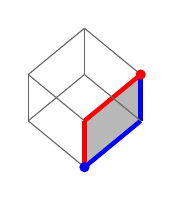
\begin{tikzpicture}%
	[	x={(0.000000cm, -1.000000cm)},
	y={(1.000000cm, 0.000000cm)},
	z={(0.000000cm, 0.000000cm)},
	scale=.5,
	back/.style={thin, color=black!60},
	edge/.style={color=black!60, thin},
	sourceedge/.style={color=red, ultra thick},
	targetedge/.style={color=blue, ultra thick},
	facet/.style={fill=black!35,fill opacity=0.800000},
	targetfacet/.style={fill=blue!80,fill opacity=0.800000},
	sourcefacet/.style={fill=red!80,fill opacity=0.800000},
	vertex/.style={inner sep=1pt,circle,draw=black,fill=black,thick},
	targetvertex/.style={inner sep=1pt,circle,draw=blue,fill=blue,thick},
	sourcevertex/.style={inner sep=1pt,circle,draw=red,fill=red,thick}]

\coordinate (-0.58824, 1.42857, -0.83333) at (-0.58824, 1.42857, -0.83333);
\coordinate (0.58824, 1.42857, 0.83333) at (0.58824, 1.42857, 0.83333);
\coordinate (1.76471, 0.00000, 0.00000) at (1.76471, 0.00000, 0.00000);
\coordinate (0.58824, 0.00000, -1.66667) at (0.58824, 0.00000, -1.66667);
\coordinate (-0.58824, -1.42857, -0.83333) at (-0.58824, -1.42857, -0.83333);
\coordinate (-1.76471, 0.00000, 0.00000) at (-1.76471, 0.00000, 0.00000);
\coordinate (-0.58824, 0.00000, 1.66667) at (-0.58824, 0.00000, 1.66667);
\coordinate (0.58824, -1.42857, 0.83333) at (0.58824, -1.42857, 0.83333);

\draw[edge,back] (0.58824, 0.00000, -1.66667) -- (-0.58824, -1.42857, -0.83333);
\draw[edge,back] (-0.58824, -1.42857, -0.83333) -- (-1.76471, 0.00000, 0.00000);
\draw[edge,back] (-0.58824, -1.42857, -0.83333) -- (0.58824, -1.42857, 0.83333);

\fill[facet] (0.58824, 0.00000, -1.66667) -- (-0.58824, 1.42857, -0.83333) -- (0.58824, 1.42857, 0.83333) -- (1.76471, 0.00000, 0.00000) -- cycle {};

\draw[targetedge] (-0.58824, 1.42857, -0.83333) -- (0.58824, 1.42857, 0.83333);
\draw[sourceedge] (-0.58824, 1.42857, -0.83333) -- (0.58824, 0.00000, -1.66667);
\draw[edge] (-0.58824, 1.42857, -0.83333) -- (-1.76471, 0.00000, 0.00000);
\draw[targetedge] (0.58824, 1.42857, 0.83333) -- (1.76471, 0.00000, 0.00000);
\draw[edge] (0.58824, 1.42857, 0.83333) -- (-0.58824, 0.00000, 1.66667);
\draw[sourceedge] (1.76471, 0.00000, 0.00000) -- (0.58824, 0.00000, -1.66667);
\draw[edge] (1.76471, 0.00000, 0.00000) -- (0.58824, -1.42857, 0.83333);
\draw[edge] (-1.76471, 0.00000, 0.00000) -- (-0.58824, 0.00000, 1.66667);
\draw[edge] (-0.58824, 0.00000, 1.66667) -- (0.58824, -1.42857, 0.83333);

\node[sourcevertex] at (-0.58824, 1.42857, -0.83333)     {};
\node[targetvertex] at (1.76471, 0.00000, 0.00000)     {};
\end{tikzpicture}
\qquad
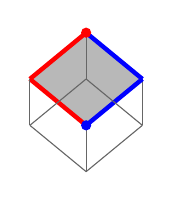
\begin{tikzpicture}%
	[x={(0.000000cm, -1.000000cm)},
	y={(1.000000cm, 0.000000cm)},
	z={(0.000000cm, 0.000000cm)},,
	scale=.5,
	back/.style={thin, color=black!60},
	edge/.style={color=black!60, thin},
	sourceedge/.style={color=red, ultra thick},
	targetedge/.style={color=blue, ultra thick},
	facet/.style={fill=black!35,fill opacity=0.800000},
	targetfacet/.style={fill=blue!80,fill opacity=0.800000},
	sourcefacet/.style={fill=red!80,fill opacity=0.800000},
	vertex/.style={inner sep=1pt,circle,draw=black,fill=black,thick},
	targetvertex/.style={inner sep=1pt,circle,draw=blue,fill=blue,thick},
	sourcevertex/.style={inner sep=1pt,circle,draw=red,fill=red,thick}]
%
\coordinate (-0.58824, 1.42857, -0.83333) at (-0.58824, 1.42857, -0.83333);
\coordinate (0.58824, 1.42857, 0.83333) at (0.58824, 1.42857, 0.83333);
\coordinate (1.76471, 0.00000, 0.00000) at (1.76471, 0.00000, 0.00000);
\coordinate (0.58824, 0.00000, -1.66667) at (0.58824, 0.00000, -1.66667);
\coordinate (-0.58824, -1.42857, -0.83333) at (-0.58824, -1.42857, -0.83333);
\coordinate (-1.76471, 0.00000, 0.00000) at (-1.76471, 0.00000, 0.00000);
\coordinate (-0.58824, 0.00000, 1.66667) at (-0.58824, 0.00000, 1.66667);
\coordinate (0.58824, -1.42857, 0.83333) at (0.58824, -1.42857, 0.83333);
%%
%%
%% Drawing edges in the back
%%

%%
%%
%% Drawing vertices in the back
%%
% \node[vertex] at (-0.58824, -1.42857, -0.83333)     {};
%%
%%
% \fill[targetfacet] (-0.58824, 0.00000, 1.66667) -- (0.58824, -1.42857, 0.83333) -- (-0.58824, -1.42857, -0.83333) -- (-1.76471, 0.00000, 0.00000) -- cycle {};
\fill[facet] (-0.58824, 1.42857, -0.83333) -- (-1.76471, 0.00000, 0.00000) -- (-0.58824, -1.42857, -0.83333) -- (0.58824, 0.00000, -1.66667) -- cycle {};
%  \fill[sourcefacet] (0.58824, 0.00000, -1.66667) -- (-0.58824, -1.42857, -0.83333) -- (0.58824, -1.42857, 0.83333) -- (1.76471, 0.00000, 0.00000) -- cycle {};


\draw[back,sourceedge] (0.58824, 0.00000, -1.66667) -- (-0.58824, -1.42857, -0.83333);
\draw[back,sourceedge] (-0.58824, -1.42857, -0.83333) -- (-1.76471, 0.00000, 0.00000);
\draw[edge,back] (-0.58824, -1.42857, -0.83333) -- (0.58824, -1.42857, 0.83333);

% %% Drawing the facets
% %%
% \fill[facet] (0.58824, 0.00000, -1.66667) -- (-0.58824, 1.42857, -0.83333) -- (0.58824, 1.42857, 0.83333) -- (1.76471, 0.00000, 0.00000) -- cycle {};
% \fill[facet] (0.58824, -1.42857, 0.83333) -- (1.76471, 0.00000, 0.00000) -- (0.58824, 1.42857, 0.83333) -- (-0.58824, 0.00000, 1.66667) -- cycle {};
%  \fill[targetfacet] (-0.58824, 0.00000, 1.66667) -- (0.58824, 1.42857, 0.83333) -- (-0.58824, 1.42857, -0.83333) -- (-1.76471, 0.00000, 0.00000) -- cycle {};
%%
%%
%% Drawing edges in the front
%%
\draw[edge] (-0.58824, 1.42857, -0.83333) -- (0.58824, 1.42857, 0.83333);
\draw[targetedge] (-0.58824, 1.42857, -0.83333) -- (0.58824, 0.00000, -1.66667);
\draw[targetedge] (-0.58824, 1.42857, -0.83333) -- (-1.76471, 0.00000, 0.00000);
\draw[edge] (0.58824, 1.42857, 0.83333) -- (1.76471, 0.00000, 0.00000);
\draw[edge] (0.58824, 1.42857, 0.83333) -- (-0.58824, 0.00000, 1.66667);
\draw[edge] (1.76471, 0.00000, 0.00000) -- (0.58824, 0.00000, -1.66667);
\draw[edge] (1.76471, 0.00000, 0.00000) -- (0.58824, -1.42857, 0.83333);
\draw[edge] (-1.76471, 0.00000, 0.00000) -- (-0.58824, 0.00000, 1.66667);
\draw[edge] (-0.58824, 0.00000, 1.66667) -- (0.58824, -1.42857, 0.83333);
%%
%%
% %% Drawing the vertices in the front
% %%
% \node[vertex] at (-0.58824, 1.42857, -0.83333)     {};
% \node[targetvertex] at (0.58824, 1.42857, 0.83333)     {};
% \node[targetvertex] at (1.76471, 0.00000, 0.00000)     {};
 \node[targetvertex] at (0.58824, 0.00000, -1.66667)     {};
 \node[sourcevertex] at (-1.76471, 0.00000, 0.00000)     {};
% \node[vertex] at (-0.58824, 0.00000, 1.66667)     {};
% \node[vertex] at (0.58824, -1.42857, 0.83333)     {};
% %%
% %%
% %
% \begin{scope}[shift={(0,3,0)}]
%
% 		%axes
% 		\draw[->] (0, 0,0) -- (1, 0,0) node[anchor=east]{$v_1$};
% 		\draw[->] (0, 0,0) -- (0, 1,0) node[anchor=west]{$v_2$};
% 		\draw[->] (0, 0,0) -- (0, 0, 1) node[anchor=west]{$v_3$};
% 	\end{scope}

\end{tikzpicture}
\qquad
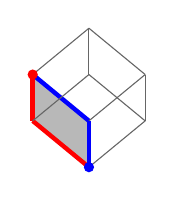
\begin{tikzpicture}%
	[x={(0.000000cm, -1.000000cm)},
	y={(1.000000cm, 0.000000cm)},
	z={(0.000000cm, 0.000000cm)},,
	scale=.5,
	back/.style={thin, color=black!60},
	edge/.style={color=black!60, thin},
	sourceedge/.style={color=red, ultra thick},
	targetedge/.style={color=blue, ultra thick},
	facet/.style={fill=black!35,fill opacity=0.800000},
	targetfacet/.style={fill=blue!80,fill opacity=0.800000},
	sourcefacet/.style={fill=red!80,fill opacity=0.800000},
	vertex/.style={inner sep=1pt,circle,draw=black,fill=black,thick},
	targetvertex/.style={inner sep=1pt,circle,draw=blue,fill=blue,thick},
	sourcevertex/.style={inner sep=1pt,circle,draw=red,fill=red,thick}]
%
\coordinate (-0.58824, 1.42857, -0.83333) at (-0.58824, 1.42857, -0.83333);
\coordinate (0.58824, 1.42857, 0.83333) at (0.58824, 1.42857, 0.83333);
\coordinate (1.76471, 0.00000, 0.00000) at (1.76471, 0.00000, 0.00000);
\coordinate (0.58824, 0.00000, -1.66667) at (0.58824, 0.00000, -1.66667);
\coordinate (-0.58824, -1.42857, -0.83333) at (-0.58824, -1.42857, -0.83333);
\coordinate (-1.76471, 0.00000, 0.00000) at (-1.76471, 0.00000, 0.00000);
\coordinate (-0.58824, 0.00000, 1.66667) at (-0.58824, 0.00000, 1.66667);
\coordinate (0.58824, -1.42857, 0.83333) at (0.58824, -1.42857, 0.83333);
%%
%%
%% Drawing edges in the back
%%

%%
%%
%% Drawing vertices in the back
%%
%%
%%
% \fill[targetfacet] (-0.58824, 0.00000, 1.66667) -- (0.58824, -1.42857, 0.83333) -- (-0.58824, -1.42857, -0.83333) -- (-1.76471, 0.00000, 0.00000) -- cycle {};
% \fill[facet] (-0.58824, 1.42857, -0.83333) -- (-1.76471, 0.00000, 0.00000) -- (-0.58824, -1.42857, -0.83333) -- (0.58824, 0.00000, -1.66667) -- cycle {};
 \fill[facet] (0.58824, 0.00000, -1.66667) -- (-0.58824, -1.42857, -0.83333) -- (0.58824, -1.42857, 0.83333) -- (1.76471, 0.00000, 0.00000) -- cycle {};


\draw[back,targetedge] (0.58824, 0.00000, -1.66667) -- (-0.58824, -1.42857, -0.83333);
\draw[edge,back] (-0.58824, -1.42857, -0.83333) -- (-1.76471, 0.00000, 0.00000);
\draw[back,sourceedge] (-0.58824, -1.42857, -0.83333) -- (0.58824, -1.42857, 0.83333);

% %% Drawing the facets
% %%
% \fill[facet] (0.58824, 0.00000, -1.66667) -- (-0.58824, 1.42857, -0.83333) -- (0.58824, 1.42857, 0.83333) -- (1.76471, 0.00000, 0.00000) -- cycle {};
% \fill[facet] (0.58824, -1.42857, 0.83333) -- (1.76471, 0.00000, 0.00000) -- (0.58824, 1.42857, 0.83333) -- (-0.58824, 0.00000, 1.66667) -- cycle {};
%  \fill[targetfacet] (-0.58824, 0.00000, 1.66667) -- (0.58824, 1.42857, 0.83333) -- (-0.58824, 1.42857, -0.83333) -- (-1.76471, 0.00000, 0.00000) -- cycle {};
%%
%%
%% Drawing edges in the front
%%
\draw[edge] (-0.58824, 1.42857, -0.83333) -- (0.58824, 1.42857, 0.83333);
\draw[edge] (-0.58824, 1.42857, -0.83333) -- (0.58824, 0.00000, -1.66667);
\draw[edge] (-0.58824, 1.42857, -0.83333) -- (-1.76471, 0.00000, 0.00000);
\draw[edge] (0.58824, 1.42857, 0.83333) -- (1.76471, 0.00000, 0.00000);
\draw[edge] (0.58824, 1.42857, 0.83333) -- (-0.58824, 0.00000, 1.66667);
\draw[targetedge] (1.76471, 0.00000, 0.00000) -- (0.58824, 0.00000, -1.66667);
\draw[sourceedge] (1.76471, 0.00000, 0.00000) -- (0.58824, -1.42857, 0.83333);
\draw[edge] (-1.76471, 0.00000, 0.00000) -- (-0.58824, 0.00000, 1.66667);
\draw[edge] (-0.58824, 0.00000, 1.66667) -- (0.58824, -1.42857, 0.83333);
%%
%%
% %% Drawing the vertices
% %%
\node[sourcevertex] at (-0.58824, -1.42857, -0.83333)     {};

% \node[vertex] at (-0.58824, 1.42857, -0.83333)     {};
% \node[targetvertex] at (0.58824, 1.42857, 0.83333)     {};
\node[targetvertex] at (1.76471, 0.00000, 0.00000)     {};
%  \node[vertex] at (0.58824, 0.00000, -1.66667)     {};
%  \node[targetvertex] at (-1.76471, 0.00000, 0.00000)     {};
% \node[vertex] at (-0.58824, 0.00000, 1.66667)     {};
% \node[vertex] at (0.58824, -1.42857, 0.83333)     {};
% %%
% %%
% %
% \begin{scope}[shift={(0,3,0)}]
%
% 		%axes
% 		\draw[->] (0, 0,0) -- (1, 0,0) node[anchor=east]{$v_1$};
% 		\draw[->] (0, 0,0) -- (0, 1,0) node[anchor=west]{$v_2$};
% 		\draw[->] (0, 0,0) -- (0, 0, 1) node[anchor=west]{$v_3$};
% 	\end{scope}

\end{tikzpicture}

\centering
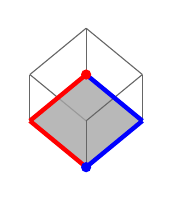
\begin{tikzpicture}%
	[x={(0.000000cm, -1.000000cm)},
	y={(1.000000cm, 0.000000cm)},
	z={(0.000000cm, 0.000000cm)},,
	scale=.5,
	back/.style={thin, color=black!60},
	edge/.style={color=black!60, thin},
	sourceedge/.style={color=red, ultra thick},
	targetedge/.style={color=blue, ultra thick},
	facet/.style={fill=black!35,fill opacity=0.800000},
	targetfacet/.style={fill=blue!80,fill opacity=0.800000},
	sourcefacet/.style={fill=red!80,fill opacity=0.800000},
	vertex/.style={inner sep=1pt,circle,draw=black,fill=black,thick},
	targetvertex/.style={inner sep=1pt,circle,draw=blue,fill=blue,thick},
	sourcevertex/.style={inner sep=1pt,circle,draw=red,fill=red,thick}]
%
\coordinate (-0.58824, 1.42857, -0.83333) at (-0.58824, 1.42857, -0.83333);
\coordinate (0.58824, 1.42857, 0.83333) at (0.58824, 1.42857, 0.83333);
\coordinate (1.76471, 0.00000, 0.00000) at (1.76471, 0.00000, 0.00000);
\coordinate (0.58824, 0.00000, -1.66667) at (0.58824, 0.00000, -1.66667);
\coordinate (-0.58824, -1.42857, -0.83333) at (-0.58824, -1.42857, -0.83333);
\coordinate (-1.76471, 0.00000, 0.00000) at (-1.76471, 0.00000, 0.00000);
\coordinate (-0.58824, 0.00000, 1.66667) at (-0.58824, 0.00000, 1.66667);
\coordinate (0.58824, -1.42857, 0.83333) at (0.58824, -1.42857, 0.83333);
%%
%%
%% Drawing edges in the back
%%

%%
%%
%% Drawing vertices in the back
%%
% \node[vertex] at (-0.58824, -1.42857, -0.83333)     {};
%%
%%
% \fill[targetfacet] (-0.58824, 0.00000, 1.66667) -- (0.58824, -1.42857, 0.83333) -- (-0.58824, -1.42857, -0.83333) -- (-1.76471, 0.00000, 0.00000) -- cycle {};
% \fill[facet] (-0.58824, 1.42857, -0.83333) -- (-1.76471, 0.00000, 0.00000) -- (-0.58824, -1.42857, -0.83333) -- (0.58824, 0.00000, -1.66667) -- cycle {};
%  \fill[facet] (0.58824, 0.00000, -1.66667) -- (-0.58824, -1.42857, -0.83333) -- (0.58824, -1.42857, 0.83333) -- (1.76471, 0.00000, 0.00000) -- cycle {};


\draw[edge,back] (0.58824, 0.00000, -1.66667) -- (-0.58824, -1.42857, -0.83333);
\draw[edge,back] (-0.58824, -1.42857, -0.83333) -- (-1.76471, 0.00000, 0.00000);
\draw[edge,back] (-0.58824, -1.42857, -0.83333) -- (0.58824, -1.42857, 0.83333);

% %% Drawing the facets
% %%
% \fill[facet] (0.58824, 0.00000, -1.66667) -- (-0.58824, 1.42857, -0.83333) -- (0.58824, 1.42857, 0.83333) -- (1.76471, 0.00000, 0.00000) -- cycle {};
\fill[facet] (0.58824, -1.42857, 0.83333) -- (1.76471, 0.00000, 0.00000) -- (0.58824, 1.42857, 0.83333) -- (-0.58824, 0.00000, 1.66667) -- cycle {};
%  \fill[targetfacet] (-0.58824, 0.00000, 1.66667) -- (0.58824, 1.42857, 0.83333) -- (-0.58824, 1.42857, -0.83333) -- (-1.76471, 0.00000, 0.00000) -- cycle {};
%%
%%
%% Drawing edges in the front
%%
\draw[edge] (-0.58824, 1.42857, -0.83333) -- (0.58824, 1.42857, 0.83333);
\draw[edge] (-0.58824, 1.42857, -0.83333) -- (0.58824, 0.00000, -1.66667);
\draw[edge] (-0.58824, 1.42857, -0.83333) -- (-1.76471, 0.00000, 0.00000);
\draw[targetedge] (0.58824, 1.42857, 0.83333) -- (1.76471, 0.00000, 0.00000);
\draw[targetedge] (0.58824, 1.42857, 0.83333) -- (-0.58824, 0.00000, 1.66667);
\draw[edge] (1.76471, 0.00000, 0.00000) -- (0.58824, 0.00000, -1.66667);
\draw[sourceedge] (1.76471, 0.00000, 0.00000) -- (0.58824, -1.42857, 0.83333);
\draw[edge] (-1.76471, 0.00000, 0.00000) -- (-0.58824, 0.00000, 1.66667);
\draw[sourceedge] (-0.58824, 0.00000, 1.66667) -- (0.58824, -1.42857, 0.83333);
%%
%%
% %% Drawing the vertices in the front
% %%
% \node[vertex] at (-0.58824, 1.42857, -0.83333)     {};
% \node[targetvertex] at (0.58824, 1.42857, 0.83333)     {};
\node[targetvertex] at (1.76471, 0.00000, 0.00000)     {};
%  \node[sourcevertex] at (0.58824, 0.00000, -1.66667)     {};
%  \node[targetvertex] at (-1.76471, 0.00000, 0.00000)     {};
 \node[sourcevertex] at (-0.58824, 0.00000, 1.66667)     {};
% \node[targetvertex] at (0.58824, -1.42857, 0.83333)     {};
% %%
% %%
% %
% \begin{scope}[shift={(0,3,0)}]
%
% 		%axes
% 		\draw[->] (0, 0,0) -- (1, 0,0) node[anchor=east]{$v_1$};
% 		\draw[->] (0, 0,0) -- (0, 1,0) node[anchor=west]{$v_2$};
% 		\draw[->] (0, 0,0) -- (0, 0, 1) node[anchor=west]{$v_3$};
% 	\end{scope}

\end{tikzpicture}
\qquad
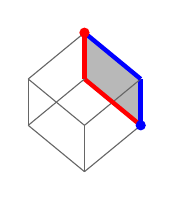
\begin{tikzpicture}%
	[x={(0.000000cm, -1.000000cm)},
	y={(1.000000cm, 0.000000cm)},
	z={(0.000000cm, 0.000000cm)},,
	scale=.5,
	back/.style={thin, color=black!60},
	edge/.style={color=black!60, thin},
	sourceedge/.style={color=red, ultra thick},
	targetedge/.style={color=blue, ultra thick},
	facet/.style={fill=black!35,fill opacity=0.800000},
	targetfacet/.style={fill=blue!80,fill opacity=0.800000},
	sourcefacet/.style={fill=red!80,fill opacity=0.800000},
	vertex/.style={inner sep=1pt,circle,draw=black,fill=black,thick},
	targetvertex/.style={inner sep=1pt,circle,draw=blue,fill=blue,thick},
	sourcevertex/.style={inner sep=1pt,circle,draw=red,fill=red,thick}]
%
\coordinate (-0.58824, 1.42857, -0.83333) at (-0.58824, 1.42857, -0.83333);
\coordinate (0.58824, 1.42857, 0.83333) at (0.58824, 1.42857, 0.83333);
\coordinate (1.76471, 0.00000, 0.00000) at (1.76471, 0.00000, 0.00000);
\coordinate (0.58824, 0.00000, -1.66667) at (0.58824, 0.00000, -1.66667);
\coordinate (-0.58824, -1.42857, -0.83333) at (-0.58824, -1.42857, -0.83333);
\coordinate (-1.76471, 0.00000, 0.00000) at (-1.76471, 0.00000, 0.00000);
\coordinate (-0.58824, 0.00000, 1.66667) at (-0.58824, 0.00000, 1.66667);
\coordinate (0.58824, -1.42857, 0.83333) at (0.58824, -1.42857, 0.83333);
%%
%%
%% Drawing edges in the back
%%

%%
%%
%% Drawing vertices in the back
%%
% \node[vertex] at (-0.58824, -1.42857, -0.83333)     {};
%%
%%
% \fill[targetfacet] (-0.58824, 0.00000, 1.66667) -- (0.58824, -1.42857, 0.83333) -- (-0.58824, -1.42857, -0.83333) -- (-1.76471, 0.00000, 0.00000) -- cycle {};
% \fill[facet] (-0.58824, 1.42857, -0.83333) -- (-1.76471, 0.00000, 0.00000) -- (-0.58824, -1.42857, -0.83333) -- (0.58824, 0.00000, -1.66667) -- cycle {};
%  \fill[facet] (0.58824, 0.00000, -1.66667) -- (-0.58824, -1.42857, -0.83333) -- (0.58824, -1.42857, 0.83333) -- (1.76471, 0.00000, 0.00000) -- cycle {};


\draw[edge,back] (0.58824, 0.00000, -1.66667) -- (-0.58824, -1.42857, -0.83333);
\draw[edge,back] (-0.58824, -1.42857, -0.83333) -- (-1.76471, 0.00000, 0.00000);
\draw[edge,back] (-0.58824, -1.42857, -0.83333) -- (0.58824, -1.42857, 0.83333);

% %% Drawing the facets
% %%
% \fill[facet] (0.58824, 0.00000, -1.66667) -- (-0.58824, 1.42857, -0.83333) -- (0.58824, 1.42857, 0.83333) -- (1.76471, 0.00000, 0.00000) -- cycle {};
% \fill[facet] (0.58824, -1.42857, 0.83333) -- (1.76471, 0.00000, 0.00000) -- (0.58824, 1.42857, 0.83333) -- (-0.58824, 0.00000, 1.66667) -- cycle {};
 \fill[facet] (-0.58824, 0.00000, 1.66667) -- (0.58824, 1.42857, 0.83333) -- (-0.58824, 1.42857, -0.83333) -- (-1.76471, 0.00000, 0.00000) -- cycle {};
%%
%%
%% Drawing edges in the front
%%
\draw[targetedge] (-0.58824, 1.42857, -0.83333) -- (0.58824, 1.42857, 0.83333);
\draw[edge] (-0.58824, 1.42857, -0.83333) -- (0.58824, 0.00000, -1.66667);
\draw[targetedge] (-0.58824, 1.42857, -0.83333) -- (-1.76471, 0.00000, 0.00000);
\draw[edge] (0.58824, 1.42857, 0.83333) -- (1.76471, 0.00000, 0.00000);
\draw[sourceedge] (0.58824, 1.42857, 0.83333) -- (-0.58824, 0.00000, 1.66667);
\draw[edge] (1.76471, 0.00000, 0.00000) -- (0.58824, 0.00000, -1.66667);
\draw[edge] (1.76471, 0.00000, 0.00000) -- (0.58824, -1.42857, 0.83333);
\draw[sourceedge] (-1.76471, 0.00000, 0.00000) -- (-0.58824, 0.00000, 1.66667);
\draw[edge] (-0.58824, 0.00000, 1.66667) -- (0.58824, -1.42857, 0.83333);
%%
%%
% %% Drawing the vertices in the front
% %%
% \node[sourcevertex] at (-0.58824, 1.42857, -0.83333)     {};
\node[targetvertex] at (0.58824, 1.42857, 0.83333)     {};
% \node[sourcevertex] at (1.76471, 0.00000, 0.00000)     {};
%  \node[sourcevertex] at (0.58824, 0.00000, -1.66667)     {};
 \node[sourcevertex] at (-1.76471, 0.00000, 0.00000)     {};
%  \node[targetvertex] at (-0.58824, 0.00000, 1.66667)     {};
% \node[targetvertex] at (0.58824, -1.42857, 0.83333)     {};
% %%
% %%
% %
% \begin{scope}[shift={(0,3,0)}]
%
% 		%axes
% 		\draw[->] (0, 0,0) -- (1, 0,0) node[anchor=east]{$v_1$};
% 		\draw[->] (0, 0,0) -- (0, 1,0) node[anchor=west]{$v_2$};
% 		\draw[->] (0, 0,0) -- (0, 0, 1) node[anchor=west]{$v_3$};
% 	\end{scope}

\end{tikzpicture}
\qquad
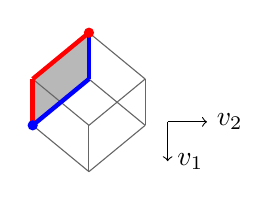
\begin{tikzpicture}%
	[x={(0.000000cm, -1.000000cm)},
	y={(1.000000cm, 0.000000cm)},
	z={(0.000000cm, 0.000000cm)},,
	scale=.5,
	back/.style={thin, color=black!60},
	edge/.style={color=black!60, thin},
	sourceedge/.style={color=red, ultra thick},
	targetedge/.style={color=blue, ultra thick},
	facet/.style={fill=black!35,fill opacity=0.800000},
	targetfacet/.style={fill=blue!80,fill opacity=0.800000},
	sourcefacet/.style={fill=red!80,fill opacity=0.800000},
	vertex/.style={inner sep=1pt,circle,draw=black,fill=black,thick},
	targetvertex/.style={inner sep=1pt,circle,draw=blue,fill=blue,thick},
	sourcevertex/.style={inner sep=1pt,circle,draw=red,fill=red,thick}]
%
\coordinate (-0.58824, 1.42857, -0.83333) at (-0.58824, 1.42857, -0.83333);
\coordinate (0.58824, 1.42857, 0.83333) at (0.58824, 1.42857, 0.83333);
\coordinate (1.76471, 0.00000, 0.00000) at (1.76471, 0.00000, 0.00000);
\coordinate (0.58824, 0.00000, -1.66667) at (0.58824, 0.00000, -1.66667);
\coordinate (-0.58824, -1.42857, -0.83333) at (-0.58824, -1.42857, -0.83333);
\coordinate (-1.76471, 0.00000, 0.00000) at (-1.76471, 0.00000, 0.00000);
\coordinate (-0.58824, 0.00000, 1.66667) at (-0.58824, 0.00000, 1.66667);
\coordinate (0.58824, -1.42857, 0.83333) at (0.58824, -1.42857, 0.83333);
%%
%%
%% Drawing edges in the back
%%

%%
%%
%% Drawing vertices in the back
%%
%%
%%
\fill[facet] (-0.58824, 0.00000, 1.66667) -- (0.58824, -1.42857, 0.83333) -- (-0.58824, -1.42857, -0.83333) -- (-1.76471, 0.00000, 0.00000) -- cycle {};
% \fill[facet] (-0.58824, 1.42857, -0.83333) -- (-1.76471, 0.00000, 0.00000) -- (-0.58824, -1.42857, -0.83333) -- (0.58824, 0.00000, -1.66667) -- cycle {};
%  \fill[facet] (0.58824, 0.00000, -1.66667) -- (-0.58824, -1.42857, -0.83333) -- (0.58824, -1.42857, 0.83333) -- (1.76471, 0.00000, 0.00000) -- cycle {};


\draw[edge,back] (0.58824, 0.00000, -1.66667) -- (-0.58824, -1.42857, -0.83333);
\draw[back,sourceedge] (-0.58824, -1.42857, -0.83333) -- (-1.76471, 0.00000, 0.00000);
\draw[back,sourceedge] (-0.58824, -1.42857, -0.83333) -- (0.58824, -1.42857, 0.83333);

% %% Drawing the facets
% %%
% \fill[facet] (0.58824, 0.00000, -1.66667) -- (-0.58824, 1.42857, -0.83333) -- (0.58824, 1.42857, 0.83333) -- (1.76471, 0.00000, 0.00000) -- cycle {};
% \fill[facet] (0.58824, -1.42857, 0.83333) -- (1.76471, 0.00000, 0.00000) -- (0.58824, 1.42857, 0.83333) -- (-0.58824, 0.00000, 1.66667) -- cycle {};
%  \fill[facet] (-0.58824, 0.00000, 1.66667) -- (0.58824, 1.42857, 0.83333) -- (-0.58824, 1.42857, -0.83333) -- (-1.76471, 0.00000, 0.00000) -- cycle {};
%%
%%
%% Drawing edges in the front
%%
\draw[edge] (-0.58824, 1.42857, -0.83333) -- (0.58824, 1.42857, 0.83333);
\draw[edge] (-0.58824, 1.42857, -0.83333) -- (0.58824, 0.00000, -1.66667);
\draw[edge] (-0.58824, 1.42857, -0.83333) -- (-1.76471, 0.00000, 0.00000);
\draw[edge] (0.58824, 1.42857, 0.83333) -- (1.76471, 0.00000, 0.00000);
\draw[edge] (0.58824, 1.42857, 0.83333) -- (-0.58824, 0.00000, 1.66667);
\draw[edge] (1.76471, 0.00000, 0.00000) -- (0.58824, 0.00000, -1.66667);
\draw[edge] (1.76471, 0.00000, 0.00000) -- (0.58824, -1.42857, 0.83333);
\draw[targetedge] (-1.76471, 0.00000, 0.00000) -- (-0.58824, 0.00000, 1.66667);
\draw[targetedge] (-0.58824, 0.00000, 1.66667) -- (0.58824, -1.42857, 0.83333);
%%
%%
% %% Drawing the vertices

% \node[targetvertex] at (-0.58824, -1.42857, -0.83333)     {};

% %%
% \node[sourcevertex] at (-0.58824, 1.42857, -0.83333)     {};
% \node[targetvertex] at (0.58824, 1.42857, 0.83333)     {};
% \node[sourcevertex] at (1.76471, 0.00000, 0.00000)     {};
%  \node[sourcevertex] at (0.58824, 0.00000, -1.66667)     {};
 \node[sourcevertex] at (-1.76471, 0.00000, 0.00000)     {};
%  \node[sourcevertex] at (-0.58824, 0.00000, 1.66667)     {};
 \node[targetvertex] at (0.58824, -1.42857, 0.83333)     {};
% %%
% %%
% %
% \begin{scope}[shift={(0,3,0)}]
%
% 		%axes
% 		\draw[->] (0, 0,0) -- (1, 0,0) node[anchor=east]{$v_1$};
% 		\draw[->] (0, 0,0) -- (0, 1,0) node[anchor=west]{$v_2$};
% 		\draw[->] (0, 0,0) -- (0, 0, 1) node[anchor=west]{$v_3$};
% 	\end{scope}
\begin{scope}[shift={(.5,2,0)}]
	\draw[->] (0, 0,0) -- (1, 0,0) node[anchor=west]{$v_1$};
	\draw[->] (0, 0,0) -- (0, 1,0) node[anchor=west]{$v_2$};
\end{scope}
\end{tikzpicture}
\\ \ \par
\end{frame}
